\documentclass[11pt, oneside]{article} 
\usepackage{geometry}
\geometry{letterpaper} 
\usepackage{graphicx}
	
\usepackage{amssymb}
\usepackage{amsmath}
\usepackage{parskip}
\usepackage{color}
\usepackage{hyperref}

\graphicspath{{/Users/telliott_admin/Tex/png/}}
% \begin{center} 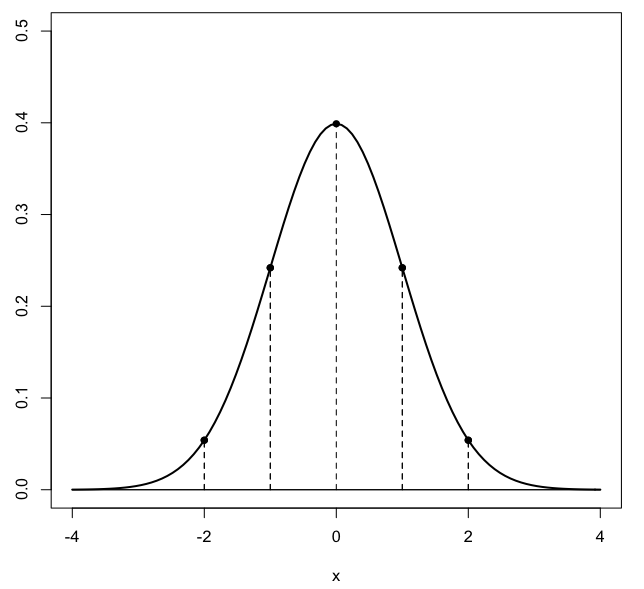
\includegraphics [scale=0.4] {gauss3.png} \end{center}

\title{Capacitor}
\date{}

\begin{document}
\maketitle
\Large

A capacitor consists of two charged objects:  parallel plates, or concentric sphere and shell.  The plates are separated by a dielectric (insulator).  A capacitor stores energy in the form of the electric field between the plates.

The potential difference is dependent on the amount of charge that is present, and physical characteristics like the size and geometry of the plates and the distance between them.

For the example of two (infinite) parallel plates, we verified elsewhere the formula for the electric field
\[ E = \frac{\sigma}{\epsilon_0} \]

This result is easy to see if we visualize an electric field with lines of flux.  By symmetry, there is nowhere to go for a line that leaves the positive plate but directly toward the negative plate.  There is no space for the lines to spread out with distance, hence, no dependence on the separation.

For a finite capacitor, if we ignore edge effects, the same basic result holds. 

The voltage difference does depend on the distance $a$ separating the plates. 
\[ V = Ea = \frac{\sigma a}{\epsilon_0} \]
 Now since $\sigma = Q/A$
\[ V = \frac{Q}{A} \ \frac{\sigma a}{\epsilon_0} \]

We consolidate all the terms except the charge into a factor $C = \epsilon_0 A/a \sigma$ so that gives
\[ V = Ea = \frac{Q}{C} \]

Capacitance $C$ relates voltage to charge
\[ CV = Q \]
The higher the capacitance, the smaller the voltage for a given amount of stored charge.  The permittivity $\epsilon_0$ changes to $\epsilon$ for other materials, where $\epsilon = k \epsilon_0$.  For example, for paper, $k=3.5$ or so.

The capacitance is defined to be the ratio of the electric charge on each conductor to the potential difference.  The unit is the farad, which is equal to one coulomb per volt.  Typical values might be microfarads $\mu F$.

A very useful property of capacitors is that they block direct current, yet allow alternating current to pass.  Also, when combined in appropriate circuits, they can be used to tune a circuit to a particular resonant frequency (e.g. in a radio).

\subsection*{energy}
If we consider a capacitor with a charge $Q$ on it, work must be done to bring a small amount of positive charge $dQ$ to the positively charged plate.  Work is equal to force times distance.

The energy stored in a capacitor can be calculated as the work done in moving a small amount of charge "from" one plate "to" another.

\[ dW = E \ dq \ a = V \ dq \]

\[ W = \int dW = \int V \ dq = \int \frac{Q}{C} \ dq \]

Hence, in building up a charge $Q$ on a capacitor the work done is just
\[ W = \frac{Q^2}{2C} = \frac{(CV)^2}{2C} = \frac{1}{2}CV^2 \]

The integral here takes account of the fact that the voltage at the time any small charge $dq$ is transferred depends on how much charge is currently on the plates.

Since current does not actually flow across the capacitor, for each electron that leaves the positive plate, one must join the negative plate.  

\subsection*{discharge circuit}
Consider a resistor $R$ and a capacitor $C$, and a switch.  The capacitor is initially charged.  Close the switch and what happens?  Use the standard rules and go around the circuit looking at the voltage drops across the components.  We get
\[ \frac{Q}{C} - IR = 0 \]

Define the current as $I = - dq/dt$, and then
\[ \frac{Q}{C} = IR = -\frac{dq}{dt} R \]

\[ \frac{dq}{Q} = -\frac{1}{RC} dt \]
\[ Q = Q_0 e^{-t/RC} \]
The charge decays exponentially with time with characteristics governed by $RC$.  In particular, if $Q = Q_0/2$ then
\[ \ln 2 = \frac{T_{1/2}}{RC} \]

The current is the time derivative of the charge
\[ I = - \frac{dq}{dt}  \]
\[ = \frac{1}{RC} Q_0 e^{-t/RC} \]
\[ = \frac{1}{RC} I_0 \]

In exactly the same way as for the charge
\[ \frac{dI}{dt} = = -\frac{1}{RC} I_0 \]
\[ RC\ \frac{dI}{dt} + I_0 = 0 \]
When you hook up a voltage and a capacitor, there is an initial current, but as the capacitor plates acquire charge the current dies away exponentially.

\subsection*{energy}
On the other hand,onsider a circuit containing a battery (or EMF $\mathcal{E}$), a resistor $R$ and a capacitor $C$, and a switch.  The capacitor is initially uncharged.  Close the switch and what happens?  Use the standard rules and go around the circuit looking at the voltage

\subsection*{series and parallel}
Everyone has probably seen the equations for resistors.
\[ V = IR \]
Put two resistors in series, and each one must carry the full current, but the voltage drop is distributed, part of it over each resistor separately.  Hence:
\[ V_{tot} = V_1 + V_2 = IR_1 + IR_2 \]
\[ = I(R_1 + R_2) = I R_{e} \]
where $R_e$ is the equivalent resistance for the two resistors together.
\[ R_1 + R_2 = R_e \]
In contrast, if the resistors are in parallel, they have the same voltage drop and the current is distributed.
\[ I = \frac{V}{R} \]
\[ I = I_1 + I_2 =  \frac{V}{R_e} \]
Thus
\[ \frac{V}{R_e} = \frac{V}{R_1} + \frac{V}{R_2} \]
\[ \frac{1}{R_e} = \frac{1}{R_1} + \frac{1}{R_2} \]
Resistances add in series, and their reciprocals add, in parallel.

Capacitors are just the opposite.  Capacitance is additive in parallel, but the reciprocals add in series.

\begin{center} 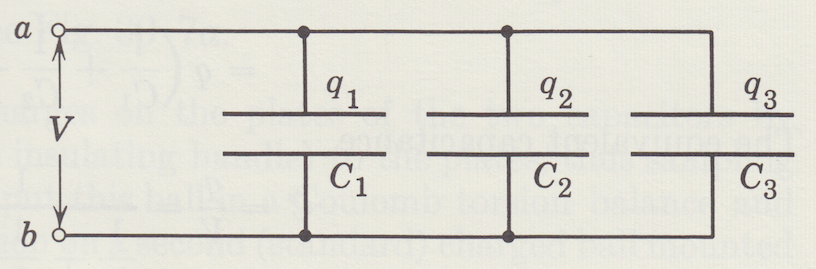
\includegraphics [scale=0.4] {capacitor_parallel.png} \end{center}

In parallel, both components have the same voltage, but the charge is additive.
\[ V = \frac{Q_1}{C_1} \]
\[ V = \frac{Q_2}{C_1} \]
\[ Q_{tot}= C_e V = C_1 V + C_2 V \]
Thus
\[ C_e = C_1 + C_2 \]

In series, the charge is the same and the voltages add
\[ V_{tot} = \frac{Q}{C_1} + \frac{Q}{C_2} = \frac{Q}{C_e} \]
\[ \frac{1}{C_1} + \frac{1}{C_2} = \frac{1}{C_e} \]

\subsection*{AC circuit}
If we put a capacitor into an AC circuit, then the charge is
\[ q(t) = CVe^{j\omega t} \]
where as before $C$ is a number that describes the capacity of the capacitor (with units of coulombs/volt), and $i$ is renamed to be $j$ because the electrical engineers use $i$ and $I$ for current.  Anyway the point is that the current across such a device is
\[ i(t) = \frac{dq}{dt} = j\omega CV e^{j\omega t} =  j\omega q(t) \]
To solve this differential equation, we need to find a function where
\[ i = \frac{dq}{dt} = j\omega q \]
If the voltage goes like the cosine, then this is a problem.

What we are going to do is to write the voltage as
\[ V(t) = V_o e^{j\omega t} \]
where $j = \sqrt{-1}$.  Then
\[ q(t) = C V_o e^{j\omega t}  \]
so the current is
\[ i(t) = j \omega C V_o e^{j\omega t}  \]
so the equivalent of the resistance for the capacitor is
\[ X_C = \frac{1}{j \omega C} \]
\[ = -\frac{j}{\omega C } \]
What does this mean?  It means that when the voltage is at the peak of its cycle, the current through the capacitor is 90 degrees out of phase with it.

\end{document}  